\section{Heavy-Tailed Self-Regularization (\HTSR)}
\label{sxn:htsr}

In this section, we provide an overview of the \HTSR \Phenomenology.%
\footnote{We may also refer to the \HTSR \Phenomenology as the \HTSR Theory; we use the term \Phenomenology to emphasize its empirical nature, and to distinguish it from the analytical methods used in the \SETOL approach.}
\HTSR has been presented in detail previously~\cite{MM19_HTSR_ICML,MM20_SDM,MM18_TR_JMLRversion}.%
\footnote{\michael{MM TO DO: Provide an overview of which papers to read, and in what order.}} 
Here, we provide a self-contained summary, with an emphasis on certain technical issues that will be important for our
\SETOL. We highlight its practical application for interpreting observed behaviors in trained weight matrices, and 
we distinguish the \HTSR \Phenomenology from the analytical methods used in the \SETOL approach.
In Section~\ref{sxn:htsr_setup}, we summarize the basic \HTSR setup and results;
in Section~\ref{sxn:guass_ht_univ}, we summarize Gaussian (for \RMT) and Heavy-Tailed (for \HTRMT) Universality; and
in Section~\ref{sxn:htsr-metics}, we describe \SHAPE metrics and \SCALE metrics that arise from \HTSR.
(Here, we focus on basic methods for identifying HT correlations in the ESDs of pre-trained weight matrices; 
in Sections~\ref{sxn:empirical-test_acc},~\ref{sxn:empirical-correlation_trap} and~\ref{sxn:hysteresis_effect}, we show detailed experiments using theoretical constructs from the \HTSR \Phenomenology.)

%%(issues that arise with spuriously HT ESDs and how to deal with them will be described in Section~\ref{sxn:HT_ESDs}).

\subsection{The \HTSR Setup}
\label{sxn:htsr_setup}

We can write the \EnergyLandscape function 
(or NN output function) for a 
%%\emph{\Typical} 
NN with $L$ layers as
\begin{equation}
\label{eqn:dnn_energy}
\NNOUT:=h_{L}(\mathbf{W}_{L}\times h_{L-1}(\mathbf{W}_{L-1}\times(\cdots)+\mathbf{b}_{L-1})+\mathbf{b}_{L}) 
\end{equation}
with activation functions $h_{l}(\cdot)$, and with weight matrices and biases $\mathbf{W}_{l}$ and $\mathbf{b}_{l}$.%
\footnote{The Energy Landscape function $\NNOUT$ acts on a data instance and generates a list of energies, or un-normalized probabilities;
~\cite{MM18_TR_JMLRversion}.
This notation was chosen to make an analogy with Random Energy Models (REM)
from spin-glass and protein folding theories~\cite{DerridaREM1981, BryngelsonWolynesPNAS1987}.
}
For simplicity of exposition here (\HTSR can be applied much more broadly), we ignore the structural details of the layers (dense or not, convolutions or not, residual/skip connections, etc.).
We also ignore the biases $b_{l}$ (because they can be subsumed into the weight matrices),
and we treat each layer as though it contains a single weight matrix $\mathbf{W}_{L}$.
We imagine training (or fine-tuning) this model on labeled data $\{\mathbf{x}_{\mu},y_{\mu}\}\in\mathcal{D}$, where $ \mathbf{x}_\mu $ is the $\mu$-th input vector and $y_\mu$ is its corresponding label (e.g., for binary classification, $y_{\mu}\in\{-1,1\}$).
We expect to use backprop via some variant of stochastic gradient descent (SGD) to minimize some loss functional, $\mathcal{L}$ (such as $\ell_2$, cross-entropy, etc.):  
\begin{equation}
\underset{\mathbf{W}_{l},\mathbf{b}_{l}}{\argmin}\;\sum_{\mu}\mathcal{L}[\NNOUT(\mathbf{x}_{\mu}),y_{\mu}]+\Omega ,
\label{eqn:dnn_opt}
\end{equation}
where $\Omega$ denotes some explicit regularizer (such as an $\ell_1$ or $\ell_2$ constraint on layer weight matrices) or some implicit regularization procedure (such as clipping the weight matrices or applying dropout).

Given a real-valued $N\times M$ layer weight matrix $\mathbf{W}$ (dropping the subscript), let $\mathbf{X}$ be the $M \times M$ layer \emph{\CorrelationMatrix}:
\begin{equation}
\mathbf{X}:=\dfrac{1}{N}\mathbf{W}^{\top}\mathbf{W} .
\label{eqn:X}
\end{equation}

\noindent
The \EmpiricalSpectralDensity (ESD) of $\mathbf{W}$, denoted $\rho^{emp}(\lambda)$, is formed from the M eigenvalues $\lambda_{j}$ of $\mathbf{X}$:
\begin{equation}
\rho_{emp}(\lambda):=\sum_{j=1}^{M}\delta(\lambda-\lambda_{j}) .
\label{eqn:rho}
\end{equation}
Given a model, we can compute the ESDs of all of its layers, as well as other metrics below,
with the open-source \WW tool~\cite{WW}.%
\footnote{For practical purposes, the \WW tool computes $\rho^{emp}(\lambda)$ by forming the Singular Value Decomposition (SVD) of the layer weight matrices $\mathbf{W}$, computing the eigenvalues $\lambda=\sigma^{2}$ from the singular values $\sigma$, and (when useful) smoothing them with a Kernel Density Estimator (KDE). For some calculations, such as the \TRACELOG condition, we must also select the appropriate normalization of $\mathbf{W}$.}


Based on empirical results based on thousands of pretrained models and tens of thousands of layers~\cite{MM18_TR_JMLRversion,MM20a_trends_NatComm,MM21a_simpsons_TR,YTHx23_KDD}, 
it is generally observed that the 
best performing NNs have ESDs that are HT, and the \emph{tails} of these ESDs, $\rho_{tail}(\lambda)$, can be well fit to a PL, beyond some cutoff $\lambda\ge\LambdaMin$.%
\footnote{Doing a large meta-analysis like this is tricky; but see~\cite{MM18_TR_JMLRversion,MM20a_trends_NatComm,MM21a_simpsons_TR,YTHx23_KDD}.  The \WW~tool provides a systematic, reproducible way to compute a PL fit (using an MLE method of Clauset et al.~\cite{CSN09_powerlaw}), as well other model metrics, including the \SPECTRALNORM, \RANDDIST, and \ALPHAHAT metrics~\cite{MM20a_trends_NatComm}.  Also, the ESD $\rho(\lambda)_{tail}$ is sometimes better fit by a Truncated \PowerLaw (TPL), due to finite-size effects.
(Again, this is important in practice, but we ignore this complexity in this initial discussion of \SETOL. ) }
For a PL fit,
\begin{equation}
\rho_{tail}(\lambda):=\rho^{emp}(\lambda\ge\LambdaMin)\sim\lambda^{-\alpha} ,
\label{eqn:rho_tail}
\end{equation}
where $\LambdaMin$ is where the tail of the ESD starts (i.e., it is not the minimum eigenvalue, but the minimum eigenvalue in the tail of the ESD). 
See Figure~\ref{fig:log-esds}.
As such, the tail of the ESD ``starts'' at some value $\LambdaMin$, called $xmin$ here, and it continues until the 
maximum eigenvalue $\LambdaMax$, called $xmax$ here
(labeled $xmax$ in the figure, shown by the orange line).
We estimate $xmin$ and $\alpha$ jointly, using the method of~\cite{CSN09_powerlaw}, 
as implemented in the \texttt{powerlaw} python package~\cite{ABP14}, 
which is also integrated into the open-source \WW tool~\cite{MM20a_trends_NatComm, WW}.%
\footnote{The authors of~\cite{Thamm2022} failed to find evidence of a PL-like distribution in NN weight matrices, which is 
likely to be the case when $\alpha$ and $xmin$ are not estimated \emph{jointly}, as can be seen in Figure~\ref{fig:xmin-DKS-esd}.  }


%%While the ESD can be computed as a histogram of eigenvalues, it is often more convenient to represent it using a kernel density estimator (KDE).


\begin{figure}[t] %[h]
    \centering
    \subfigure[Log-Log ESD]{
      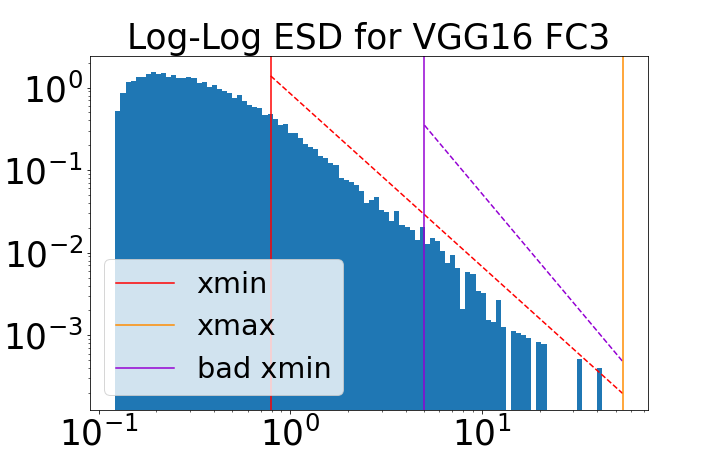
\includegraphics[width=7cm]{./img/fig1-1a.png}
      \label{fig:log-log-esd}
    }
    \subfigure[Lin-Lin ESD]{
      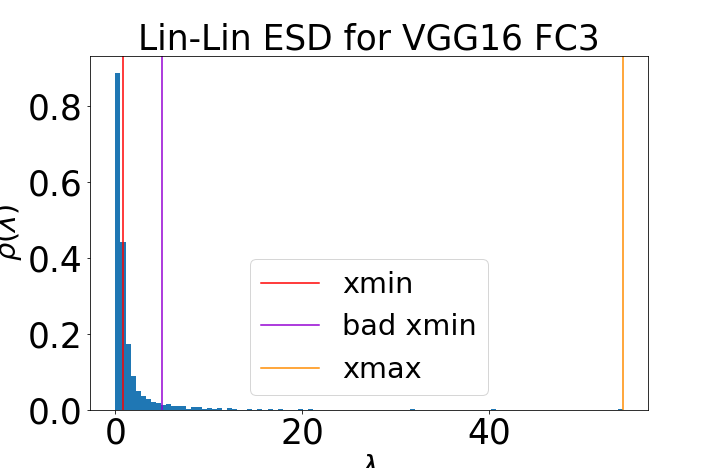
\includegraphics[width=7cm]{./img/fig1-1b.png}
      \label{fig:lin-lin-esd}
    }
    \subfigure[Log-Lin ESD]{
      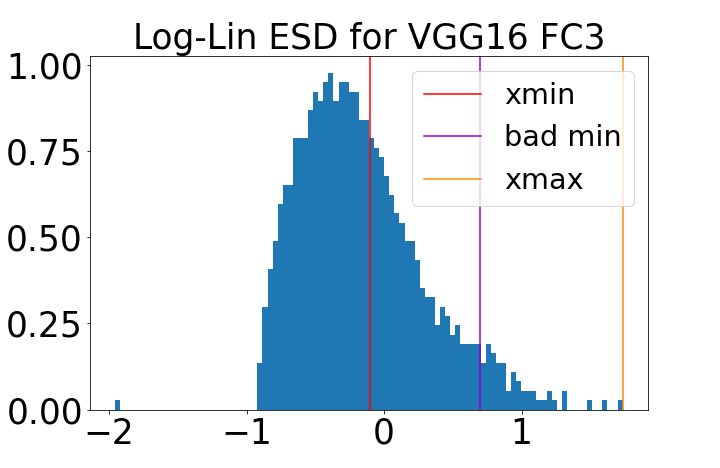
\includegraphics[width=7cm]{./img/fig1-1c.png}
      \label{fig:log-lin-esd}
    }
    \subfigure[$\LambdaMin$ vs KS distance]{
      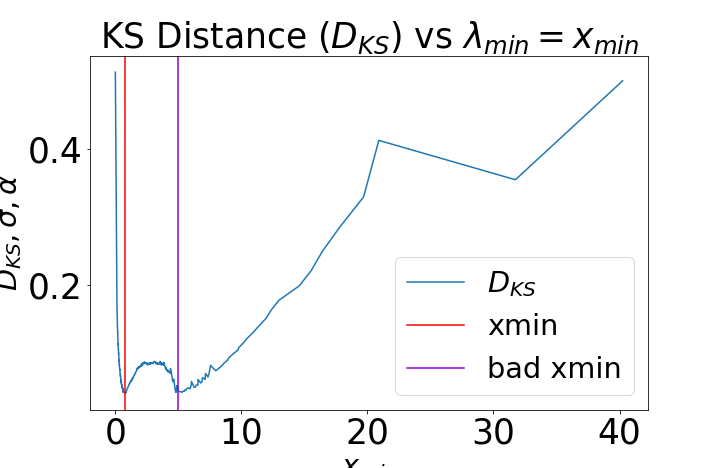
\includegraphics[width=7cm]{./img/fig1-1d.png}
      \label{fig:xmin-DKS-esd}
    }                                     
    \caption{\textbf{Fitting ESDs within \HTSR.} 
         Depiction of the ESD and results of PL fits for a typical well-trained layer of a modern NN (FC3 of VGG19), including both the actual and good PL fit (red) and a hypothetical bad PL fit (purple). 
         The same ESD is plotted on a Log-Log (a), Lin-Lin (b) and Log-Lin (c) scales.
         (d) depicts how the start of the PL tail, $\LambdaMin$, varies with the quality of the PL fit (the $D_{KS}$ distance). 
         All plots are generated using the open-source \WW tool. 
         See the main text for details.
    }
  \label{fig:log-esds}
\end{figure}   


%% %Figure~\ref{fig:log-esds} (from Figure~1 of~\cite{MM21a_simpsons_TR}) displays layer ESD plots for a \Typical layer $\mathbf{W}$,
%% %on different scales (\ref{fig:log-log-esd}, \ref{fig:lin-lin-esd}, \ref{fig:log-lin-esd}),
%% %along with the quality of fit ($D_{KS}$ vs. $x_min$, \ref{fig:xmin-DKS-esd}), as generated with the~\WW~tool,
%% %\footnote{The \WW~tool finds the best PL fit automatically and reproducibly.}

\paragraph{Fitting ESDs.}
Choosing the start of the tail, $\LambdaMin$, is important for \HTSR (and it will be very important for \SETOL, as we will describe below).
See Figure~\ref{fig:log-esds} for a depiction of how this was done within \HTSR theory.
Figures~\ref{fig:log-log-esd}-\ref{fig:log-lin-esd} show the results of both a ``good fit'' and a ``bad fit'' on the same ESD,
while Figure~\ref{fig:xmin-DKS-esd} indicates the quality of fit.
For the good fit, the start of the tail is the optimal value $\LambdaMin=xmin$ (in red); and for the bad fit, it is a suboptimal $bad\;xmin$ (purple).
Figure~\ref{fig:xmin-DKS-esd} depicts how the best fit is determined; it plots $xmin=\LambdaMin$ versus the $D_{KS}$ 
value, which is the Kolmogorov-Smirnov (KS) distance between the PL fit and the empirical data~\cite{CSN09_powerlaw}.
Notice that there are two nearly degenerate minima on Figure~\ref{fig:xmin-DKS-esd}, corresponding to the good fit and the bad fit. 
It is not uncommon to face such practical challenges, as real-world ESDs are often slightly deformed from a perfect PL density, e.g.,
they may have two or more near-degenerate solutions on the KS plots (d).
(They may also have anomalously large eigenvalues; this is discussed in more detail in Section~\ref{sxn:HT_ESDs}.)

When one finds a good PL fit for the ESD of a layer $\mathbf{W}$,
it provides information about the \SHAPE~and \SCALE~of the ESD of that layer.
In particular: 
the \SPECTRALNORM, $\lambda_{max}$, being a matrix norm, is a measure of the size \SCALE~of the ESD~\cite{MM21a_simpsons_TR}; 
the fitted PL exponent \ALPHA, $\alpha$, being the slope of the tail of the ESD on a Log-Log plot, describes the \SHAPE~of the ESD; and
the \WW \ALPHAHAT~metric combines \SHAPE~and \SCALE~information.
Also, as opposed to other applications of PL fits~\cite{CSN09_powerlaw,BouchaudPotters03}, in our analysis,
the start of the tail, $\LambdaMin=\LambdaPLmin$, plays a particularly important role because it
identifies the subspace of the strongest generalizing eigencomponents (i.e., $\XECS$, below) in each layer.

\begin{table}[t] %[ht!]
\begin{center}
  \begin{tabular}{| l | c | c | r | }
    \hline
    HT/\RMT Universality class & $\mu$ range   & $\alpha$ range    & Best Fit  \\ \hline \hline
    RandomLike            & NA            & NA                & MP        \\ \hline
    Bulk+Spikes           & NA            & NA                & MP+Spikes \\ \hline
    Weakly Heavy Tailed   & $\mu > 4$     & $\alpha>6$        & PL        \\ \hline
    Heavy (Fat) Tailed    & $\mu\in(2,4)$ & $\alpha\in(2,6)$  & PL        \\ \hline
    Very Heavy Tailed     & $\mu\in(0,2)$ & $\alpha\in(1,2) $ & (T)PL     \\ \hline
    Rank Collapse       & NA            & NA                & NA        \\ \hline
  \end{tabular}
\end{center}
\caption{\HTSR~Heavy-Tailed Universality classes of \RMT. See Table~1 of \cite{MM18_TR_JMLRversion} for more details.    }
\label{tab:Uclass}
\end{table}



\subsection{Gaussian and Heavy-Tailed Universality}
\label{sxn:guass_ht_univ}

The \HTSR \Phenomenology uses \RMT to classify of the ESD of a layer $\mathbf{W}$ into one of 5+1 Phases of Training, 
each roughly corresponding to a (Gaussian or HT) Universality class (of \RMT or \HTRMT).
This is summarized in Table~\ref{tab:Uclass}. 
A Universality class is a set of matrices having a common limiting spectral distribution, regardless of the other properties of their entries. 
Of those, the most familiar is the Gaussian class, characterized by the Marchenko Pastur (MP) results from traditional \RMT~\cite{EW13,potters_bouchaud_2020}. 
The Gaussian Universality class, however, is particularly poorly suited for analyzing realistic NNs---precisely
because the ESDs of SOTA NNs are well-fit by HT distributions.
This should not be surprising: weight matrices of realistic NNs do \emph{not} have independent (i.i.d.)
entries---their entries are strongly-correlated precisely because they provide a view into the correlated training data.

To model strongly-correlated NN layer matrices, the \HTSR \Phenomenology characterizes NN layer weight matrices
in terms of their ESDs (when a good PL fit can be found) by postulating that the (tail of the) eigenvalue spectrum $\rho(\lambda)$ 
determines how each layer contributes to the overall generalization.  
To do this, the \HTSR approach models the strong-correlated layer weight matrices \emph{as if} they are actually i.i.d. HT random
(i.e., entry-wise uncorrelated) matrices. 
By doing this, one can  associate each $\rho(\lambda)$ with 
the corresponding HT Universality class, according to the PL exponent $\alpha$ fitted from the ESD. 
As we will see in 
Section~\ref{sxn:HT_ESDs}, it can be critical to distinguish  when the ESD is HT\emph{Correlation-wise} vs HT \emph{Element-wise}.
\michael{MM TO DO: refine that sentence, in light of similar such changes I'll make above.}

To understand Table~\ref{tab:Uclass} better, we first review basic results.  %% from (Gaussian and HT) \RMT.


\subsubsection{\RandomMatrixTheory (\RMT):  Marchenko-Pastur (MP) Theory and Tracy-Widom (TW) Fluctuations}

\begin{figure}[t] %[h]
    \centering  
    \subfigure[MP, varying $Q=\tfrac{N}{M}$]{ 
      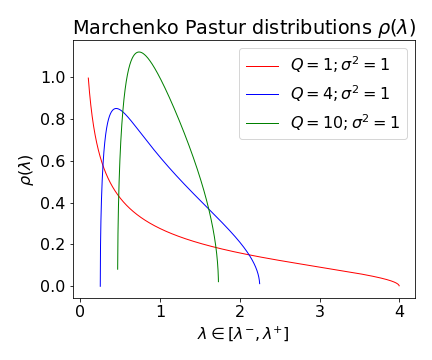
\includegraphics[width=7.0cm]{./img/mp-Q.png}
      \label{fig:MP-esds-a}
    }                               
    \subfigure[Tracy Widom fluctuations]{
      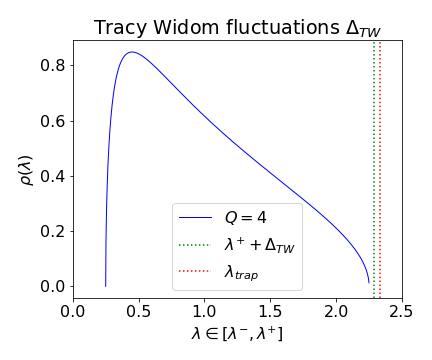
\includegraphics[width=7.0cm]{./img/mp-TW.png}
      \label{fig:MP-esds-b}
    }                    
    \caption{MP distributions for different aspect ratios $Q$ and variance scales $\sigma^2$, and an example of the finite-sized TW fluctuation $\Delta_{TW}$. }
   \label{fig:MP-esds}
\end{figure}

The Marchenko-Pastur (MP) distribution predicts the (limiting) \SHAPE of an ESD, $\rho_{MP}(\lambda)$, when the layer weight matrix has elements that are i.i.d. random from the Gaussian \Universality class.
%%As such, \HTSR theory is particularly useful when the ESD deviates from the MP predictions.
In particular, the ESD will be MP when the matrix elements are drawn from a Normal distribution $W_{i,j}\in  N(0,\sigma^{2})$, e.g., as is typical at initialization, before NN training begins.
Figure~\ref{fig:MP-esds} (from Figure~4 of \cite{MM18_TR_JMLRversion}) displays the MP distribution for different aspect ratios $Q=\tfrac{N}{M}$ and variances $\sigma^{2}$.  
Notice that the \SHAPE is characterized by a well-defined, compact envelope with sharp edges.

The MP distribution also predicts the \SCALE of an ESD, again when the layer weight matrix has elements that are i.i.d. random from the Gaussian \Universality class.
In particular, an MP distribution, $\rho_{MP}(\lambda)$, has very crisp, well-defined lower and upper bounds $\lambda^{-},\lambda^{+}$~\cite{MM18_TR_JMLRversion}, and (importantly) the upper bound $\lambda^{+}$ exhibits finite-size Tracy-Widom (TW) fluctuations, $\Delta_{TW}(\lambda)$, which are on the order of $\mathcal{O}(M^{-2/3})$. 
Thus, any layer eigenvalue with \SCALE greater than this, i.e., $\lambda>[\lambda^{+}+\Delta_{TW}(\lambda)]$, is an ``outlier'' or a ``spike.''

According to the \HTSR \Phenomenology, these spikes carry significant generalizing information. 
(This is well-known for Bulk-Plus-Spike models~\cite{MM18_TR_JMLRversion}, but the \HTSR \Phenomenology generalizes this concept.)
%
Relatedly, for layer matrices $\mathbf{W}$ with aspect ratio $Q>1$ (i.e., rectangular matrices, where $N>M$), MP \RMT predicts there should be no zero eigenvalues, i.e., $\lambda_i>0$, for all $i$. 
Generally speaking, for well trained NNs, for layers with $Q>1$, all eigenvalues are strictly larger than zero, i.e., 
well-trained layer weight matrices, with $Q>1$, should have full rank and exhibit no ``rank collapse.'' 
\michael{MM TO DO: that sentence needs to go elsewhere.}
\HTSR places random Gaussian and ``Bulk-Plus-Spike'' matrices into the first two rows of Table~\ref{tab:Uclass}.
The essential feature of Gaussian random matrices is that their entries have no correlations. 
When some correlations are injected, a few large spike eigenvalues form, without otherwise disturbing the shape of the ESD. 
\michael{MM TO DO: put in comment about how bulk-plus-spike is just a perturbative variant of MP.}
To really understand how individual NN layers converge, we need to understand when and why their ESDs become HT.


\subsubsection{\HeavyTailed \RandomMatrixTheory (\HTRMT) and \PowerLaw (PL) fits}
\label{sxn:htsr_pl_fits}

For very well-trained NN layers, ESDs are \emph{not} MP at all.
Frequently, if not always, their ESDs are HT---and they are HT \emph{because} they are strongly-correlated matrices.  
Importantly, they are \emph{not} HT element-wise.
Instead, their entries have a scale, and they have ESDs that are HT due to correlations learned during training. 
Existing theoretical approaches, including \SLT and even \STATMECH, cannot readily model such strongly-correlated systems.%
\footnote{For example, such theoretical approaches typically deal better with \emph{\Scale} information (such as $\lambda_{max}$) than with 
\emph{\Shape} information (such as $\alpha$), e.g., by characterizing an ``eigen-gap'' separating large eigenvalues from 
``noise''~\cite{bach2006_JMLR} according to a noise plus low-rank perturbation model~\cite{BFR11}.}

Such strongly-correlated systems, however, do frequently arise in other, related scientific domains, including
in the \STATMECH of self-organizing systems~\cite{bak97a,SornetteBook}, 
in electronic structure theory~\cite{Martin1996,Martin1998,Martin1996_CPL}, and
in quantitative finance~\cite{bouchaud1999,bouchaud2005,potters_bouchaud_2020}. 
In these (and other) domains, correlated systems frequently exhibit characteristic PL signatures; and it is common practice to \emph{model} correlated systems as random (uncorrelated) systems by using HT statistics (e.g., Levy distributions or PL random matrices), fully understanding that such systems are by no means actually i.i.d. random.
The \HTSR \Phenomenology builds upon this longstanding practice by 
%providing a qualitative \Phenomenology that characterizes the layers in well-trained NNs.
delimiting families of HT NN weight matrices based on the corresponding Universality classes of Pareto matrices. 

We explain briefly how to interpret Table~\ref{tab:Uclass} with respect to \HTRMT. The 5+1 Phases of Training can be 
identified by fitting ESDs to MP or PL distributions, whichever gives the best fit, as shown in the last column.
In case the PL distribution is a better fit, \HTSR \Phenomenology treats the layer weight matrix as 
equivalent to an i.i.d. random matrix $\mathbf{W}(\mu)$, whose elements have been drawn from a Pareto distribution 
with exponent $\mu$. 

\paragraph{Heavy-Tailed Universality Classes of Random Pareto Matrices}
For such an element-wise HT matrix, the theoretical \emph{limiting} ESD of a Pareto matrix is also PL,
which allows us to related the fitted PL $\alpha$ with exponent $\alpha=a\mu+b$, to the Pareto exponent $\mu$.
Ideally, for an infinite width matrix ,  $a=\tfrac{1}{2}$ and $b=1$, but due to finite-size effects, however,
we have found we must take $a\ge \tfrac{1}{2}$ and $b\ge 1$, giving
\begin{align}
W_{i,j}(\mu)\sim\dfrac{C}{x^{\mu +1}},\;\;\;\rho(\lambda)\sim\lambda^{-(a\mu+b)}.
\end{align}
According to the above relation, 
we can use either the fitted PL exponent $\alpha$, or the Pareto exponent $\mu$,
to index the HT Universality classes,
Note, however, that the finite-size effects strongly depend on  the and aspect ratio  $Q=N/M$,
at least when applied to i.i.d random Pareto matrices, and 
the (Clauset MLE) PL fit may overestimate the $\alpha$ of the ESD.
Table~\ref{tab:Uclass} delimits the HT matrices 
into sub-categories (as shown in the bottom four rows)  based on the behaviors of $\alpha$ as a function of $\mu$.

Figure~\ref{fig:HT-esds} illustrates how the fitted PL exponent $\alpha$ corresponds to the actual Pareto exponent $\mu$ 
for different aspect ratios $Q=M/M$.
Figure~\ref{fig:HT-esds-a} displays the ESDs of three different i.i.d. $1000\times1000$ HT random matrices, with $\mu=1,3,5$, on a Log-Log scale.  
Notice that smaller $\mu$, and therefore smaller $\alpha$, corresponds to heavier (i.e., larger) tails.
Figure~\ref{fig:HT-esds-b} shows how the empirically fit PL exponent $\alpha$ can vary with the theoretical $\mu$ for an associated $\mathbf{W}(\mu)$.
For $\mu<2$ and $Q=1$, the fitted $\alpha$ follows the linear relation $\alpha=\frac{1}{2}\mu+1$,
albeit with some error.
In contrast, for the more relevant $\mu \in (2,4)$ regime, the relation now depends far more 
strongly on the aspect ratio $Q$, and $\alpha\in[2,6]$.
For $\mu>4$, the fitted $\alpha$ saturates for each specific value of $Q$.

We emphasize that we only model the ESDs of the NN layer weight matrices using the
same Universality class to that associated with the ESD of a random, i.i.d, HT Pareto matrix.
In fact, the elements $W_{i,j}$ do not at all appear as if they have been
drawn from an HT Pareto distribution, and, in contrast, are almost always well fit to a Laplacian distribution.
Also, despite these strong finite-size effects, empirically one finds that the ESDs arising large, well trained,
modern NNs can frequently be well fit to a PL (or TPL), and that the fitted $\alpha\in [2,6]$ for $80-90\%$
of NN layers.  Notably, we rarely find $\alpha<2$ in the best performing, open source, pretrained DNNs.

\charles{Not sure where to put this..see text also}
%Despite the fact that Correlation-wise HT matrices found in NNs and Element-wise HT Pareto matrices arrive at their
As there is \emph{no} ground truth whatsoever as to the limiting spectral density of a strongly-correlated NN weight matrix
(especially without HT elements)
the \HTSR \Phenomenology uses Pareto matrices as a guide. 
However, as we will see in Section~\ref{sxn:HT_ESDs}, this analogy should be treated with caution because there are 
cases where it breaks down.

No matter why a matrix ESD is HT, it can be difficult to reliably estimate the $\alpha$ parameter when
the true $\alpha$ is large. For Pareto matrices of the size investigated here, 
an observed $\alpha$ above $6$ is uninformative --- the tail will decay very rapidly indeed,
leaving very little of it to study.
In this sense, the HT Universality classes are \emph{larger} than the set of only strongly-correlated 
matrices or Pareto random matrices.



%and they can be used to model the strongly-correlated weight matrices $\mathbf{W}$---as long as we are careful to distinguish 
%between when $\mathbf{W}$ is element-wise HT and when $\mathbf{X}$ is correlation-wise HT. 
%HT because $\mathbf{W}$ is strongly-correlated.

\begin{figure}[h]
    \centering  
    \subfigure[Heavy Tailed ESDs]{ 
      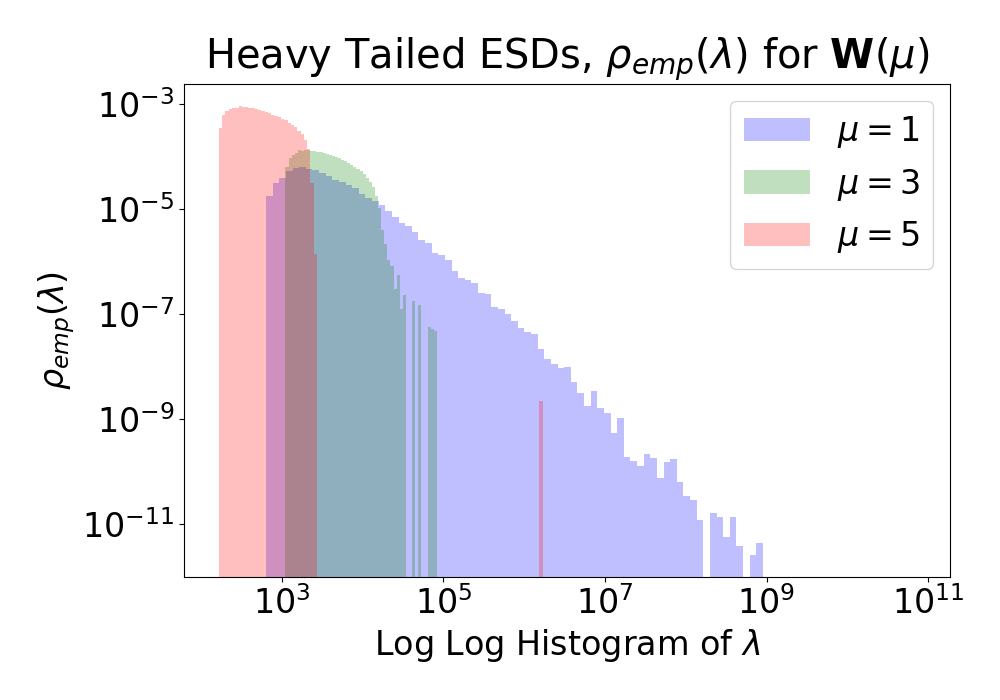
\includegraphics[width=7cm]{./img//heavy-tailed-log-log-esds.png}
      \label{fig:HT-esds-a}
    }                               
    \subfigure[PL $\alpha$ vs HT $\mu$ exponent]{
      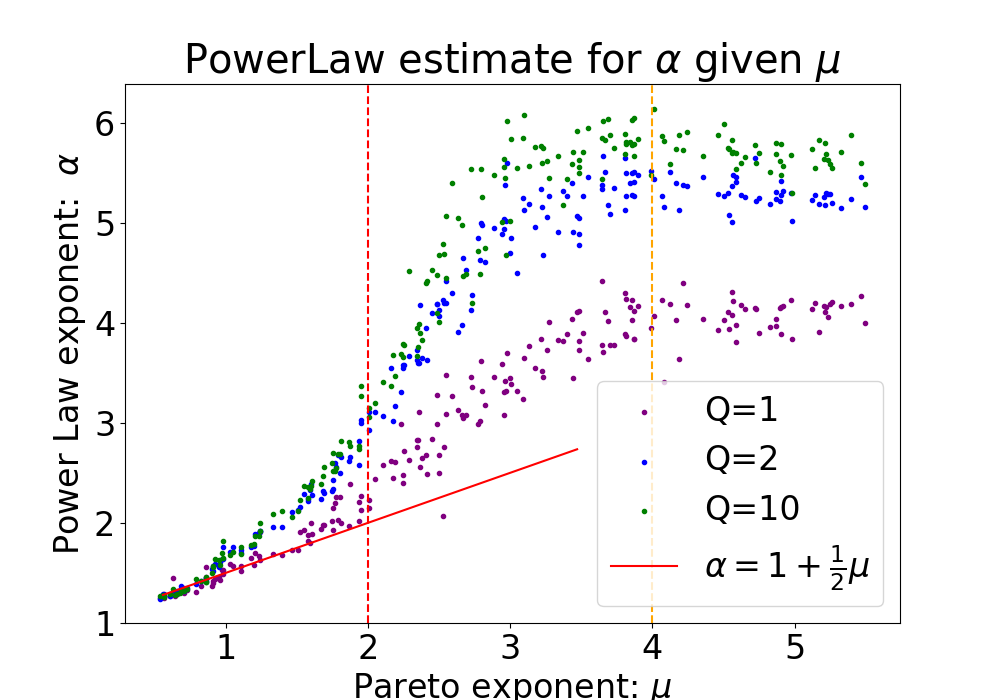
\includegraphics[width=7cm]{./img/alpha-mu-plot2.png}
      \label{fig:HT-esds-b}
    }                                                                                                                            
    \caption{Comparison of ESDs and Power Law (PL) exponents $\alpha$ from Heavy-Tailed (Pareto) 
weight matrices $\mathbf{W}(\mu)$. 
Subfigure (a) depicts 3 \Typical ESDs with Pareto exponent $\mu=1,3,5$, each decreasing in \SHAPE~and \SCALE.
Subfigure (b) shows how the exponent $\alpha$ of the PL fit varies with $\mu$, with significant finite-size
effects emerging for $\mu>2$ and $\alpha>2$.
}
   \label{fig:HT-esds}
\end{figure}

There is a particularly important boundary between Universality classes where $\alpha = 2$. Recall that one of the 
properties of power law distributions $\rho(\lambda)\sim \lambda^{-\alpha}$ is that if $\alpha<2$, than the variance of 
$\rho(\lambda)$ is infinite. In such cases, the variance cannot be estimated empirically, making $\rho(\lambda)$ in 
some sense \emph{\ATypical}. This implies that the NN will have substantially greater difficulty in applying any further 
load to such a weight matrix. Thus, the value of $\alpha = 2$ is a \emph{critical value}. (See 
Figure~\ref{fig:mlp3-FC1-alpha-overloaded} in Section~\ref{sxn:hysteresis_effect} for an empirical study of this effect 
in a small MLP.)

%When fitting ESDs of well-trained models, 
Smaller PL exponent $\alpha$ values correspond to heavier tails, $\rho_{tail}(\lambda)$; and
the \HTSR \Phenomenology observes that smaller PL exponents $\alpha$ (at least for $\alpha\in(2,6)$) tend to correspond to better models.
This is the key idea of the \HTSR:
the generalizing components of a layer matrix $\mathbf{W}$ concentrate in larger singular vectors associated with the tail, and 
so that better models have more slowly-decaying (i.e., larger) ESD tails.
This differs significantly than simply taking a general low-rank approximation to $\mathbf{W}$, where the rank
is chosen without insight from the \HTSR \Phenomenology. 
The \SETOL theory formalizes this observation as a key assumption. We will revisit these model selection questions in 
Section~\ref{sxn:setol_overview} below.




\subsection{Data-Free \SHAPE and \SCALE \Quality Metrics}
\label{sxn:htsr-metics}

The \HTSR \Phenomenology provides quality metrics for both individual layers and (by averaging layers) for an entire NN model.

\paragraph{Layer-wise Quality Metrics.}
Using the \HTSR \Phenomenology, we can define several other \SHAPE and/or \SCALE based layer (quality) metrics.
These are available in the \WW tool, and they work very well in practice.
\begin{itemize}
\item 
\ALPHA 
$(\alpha)$: $\rho_{tail}(\lambda)\sim\lambda^{-\alpha}$. 
A \SHAPE-based quality metric.
\item
\LOGSPECTRALNORM: $\log_{10}\lambda_{max}$.
A \SCALE-based quality metric.
\item 
\ALPHAHAT 
$(\hat{\alpha})$: $\alpha\log_{10}\lambda_{max}$.
A \SCALE-adjusted \SHAPE-based quality metric.
\item
\RANDDIST: $JSD[\rho^{emp}|(\rho_{rand}^{emp})]$.
A \SHAPE-based, non-parametric quality metric, suitable for highly-accurate, epoch-by-epoch analysis.%
\footnote{JSD is the Jensen-Shannon Divergence between the original ESD and the ESD of the layer weight matrix, randomized element-wise.}
\item
\PLKS: $D_{KS}$.
The KS-distance, or quality-of-fit, of the PL fits.  
For transformers, foundation models, and large, complex, modern NNs, this is frequently an even better model quality metric than the $\alpha$ of the PL fit itself.
\item
\MPSOFTRANK: $\mathcal{R}_{MP}$.
The MP-SoftRank, defined in~\cite{MM18_TR_JMLRversion}, can be used to identify problems such as when there is significant label or data noise that causes spuriously small $\alpha$, and also when it is difficult to fit a PL law.%
\footnote{The~\WW tool also implements the WW-SoftRank, which is like the MP-SoftRank, but replaces $\lambda_{bulk}^{+}$ with $\lambda_{rand}^{max}$; these are mostly equivalent for large matrices, but they can be different for very small matrices.}
\end{itemize}

\noindent
Each of these quality metrics provides a simple characterization of the \SHAPE and/or \SCALE of the tail of the ESD of a given layer $\mathbf{W}$.
These metrics are related to each other, and they have various trade-offs in practice~\cite{MM20a_trends_NatComm, MM21a_simpsons_TR, YTHx23_KDD}.
Of particular interest here in our development of \SETOL are the PL-based \WW~\ALPHA and  \ALPHAHAT~metrics.


\paragraph{From Layer-wise Quality Metrics to Layer-Averaged Model Quality Metrics.}
One can use the \HTSR \Phenomenology to go beyond individual \LayerQuality metrics, to construct model quality metrics by averaging \LayerQuality metrics (over all layers that are not very small). 
%%The PL \ALPHA and  \ALPHAHAT metrics in particular correlate remarkably well with reported test accuracies for a wide range of large and very well trained NN models~\cite{MM20a_trends_NatComm,MM19a_TR}.
Existing \HTSR model quality metrics implicitly require that all layers are statistically independent, so that the average model quality is just the average of the contributions from each weight matrix $\mathbf{W}$.%
\footnote{This independence assumption, clearly a mathematical convenience, gets us closer to a workable theory. One could go beyond a ``single layer theory'' by adding in intra-layer correlations empirically. The \WW tool does support this, but doing so is outside the scope of this work.}
%
Given a \LayerQuality metric, $\Q^{NN}_{L}(\mathbf{W})$, one can define the \emph{\ModelQuality} $\Q^{NN}$ metric for an entire model as 
\begin{align}
\label{eqn:ProductNorm}
\Q^{NN}&:=\underset{L}{\prod}\;\Q^{NN}_{L}(\mathbf{W}) ,
\end{align}
a product of each independent \LayerQuality $\Q^{NN}_{L}$, and then consider the layer average as the log \emph{\LayerQuality},
\begin{align}
\label{eqn:LogProductNorm}
\log\Q^{NN}=\frac{1}{N_{L}}\underset{L}{\sum}\;\log\Q^{NN}_{L}=\langle\log\Q^{NN}_{L}\rangle_{\bar{L}}
\end{align}
where $\langle\;\cdots\;\rangle_{\bar{L}}$ denotes the layer average.

In particular, prior work has used the following metrics:
\begin{itemize}
\item
The layer-averaged model quality metric \ALPHA, $\log\Q^{NN}=\langle\alpha\rangle_{\bar{L}}$, describes the \SHAPE of the ESDs.
One can use the averaged \ALPHA when studying a single model, and only varying the regularization hyperparameters, although \ALPHA also works very well as a model quality metric when comparing different transformer models~\cite{YHTx21_TR}.
\item
The layer-averaged model quality metric \LOGSPECTRALNORM, $\log\Q^{NN}=\langle\log\lambda_{max}\rangle_{\bar{L}}$, describes the \SCALE of the ESDs.
The averaged \LOGSPECTRALNORM does work as a model quality metric but not as well as \ALPHA~(or \ALPHAHAT).
Notably, \SLT predicts that smaller, not larger, \LOGSPECTRALNORM should be correlated with model quality; the opposite is observed in practice!
This is because smaller layer $\alpha$ generally, but not always, corresponds to larger $\lambda_{max}$.%
\footnote{The \LOGSPECTRALNORM can exhibit a Simpson's paradox when segmenting models by quality)~\cite{MM21a_simpsons_TR}.  Nevertheless, this metric may be useful when a PL fit can not be obtained, say, when $N\gg M$ and $M$ is very small, as with LSTMs,  U-Net architectures, etc.}
\item
The layer-averaged model quality metric \ALPHAHAT, $\log\Q^{NN}=\langle\alpha\log\lambda_{max}\rangle_{\bar{L}}=\langle\hat{\alpha}\rangle_{\bar{L}}$, incorporates both \SHAPE and \SCALE information.
This can compensate for anomalies that can arise when (say) comparing models of different sizes or model qualities~\cite{MM21a_simpsons_TR} or when other issues cause unusually large $\lambda_{max}$. See Section~\ref{sxn:Traps}).
\end{itemize}

\noindent
The layer-averaged \ALPHAHAT model quality metric has been applied in a large meta-analysis of hundreds of SOTA 
pre-trained publicly-available NN models in CV and NLP~\cite{MM20a_trends_NatComm,YTHx22_TR,YTHx23_KDD,MM19a_TR}. 
%
Generally speaking, \HTSR shape-based metrics, when used appropriately, outperform all other metrics studied (including 
those from \SLT, and with access to the training/testing data,) for predicting the quality of SOTA pre-trained publicly-available NN models.  
%
The \HTSR theory predicts that the best-performing NN models have layers with $\ALPHA\in[2,6]$, and with $\alpha=2$
indicating optimal performance.
Moreover, prior empirical results show that the \ALPHA and \ALPHAHAT~metrics can predict trends in the \Quality 
(i.e., the \GeneralizationAccuracy), of SOTA NN models---\emph{even without access to any training or testing data}~\cite{MM20a_trends_NatComm}.
\michaeladdressed{Somewhere, around here, we need to be more explicit that we want $\alpha$ in $[2,4]$, with lower better, and that for \HTSR the latter comes from more of an informal argument from other areas that we squeeze more juice from the data; but it is not derived, even semi-empirically, from an underlying theory.}




